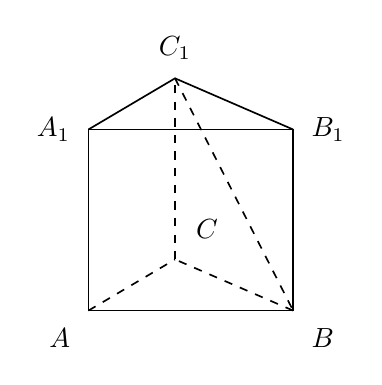
\begin{tikzpicture}[x=1cm,y=1cm,line width=.6pt]
\coordinate (A) at (0,0);
\coordinate (B) at (2.6,0);
\coordinate (Cc) at (1.1,0.65);
\coordinate (A1) at (0,2.3);
\coordinate (B1) at (2.6,2.3);
\coordinate (C1) at (1.1,2.95);
% front face solid
\draw (A) -- (B) -- (B1) -- (A1) -- cycle;
% top edges to C1
\draw (A1) -- (C1) -- (B1);
% bottom hidden to C
\draw[dashed] (A) -- (Cc);
\draw[dashed] (B) -- (Cc);
% lateral C-C1 hidden
\draw[dashed] (Cc) -- (C1);
% space diagonal C1-B
\draw[dashed] (C1) -- (B);
% labels
\node[below left=3pt,font=\normalsize] at (A) {$A$};
\node[below right=3pt,font=\normalsize] at (B) {$B$};
\node[above right=4pt,font=\normalsize] at (Cc) {$C$};
\node[left=3pt,font=\normalsize] at (A1) {$A_{1}$};
\node[right=3pt,font=\normalsize] at (B1) {$B_{1}$};
\node[above=3pt,font=\normalsize] at (C1) {$C_{1}$};
\end{tikzpicture}
